\begin{figure}[H]
	\centering
	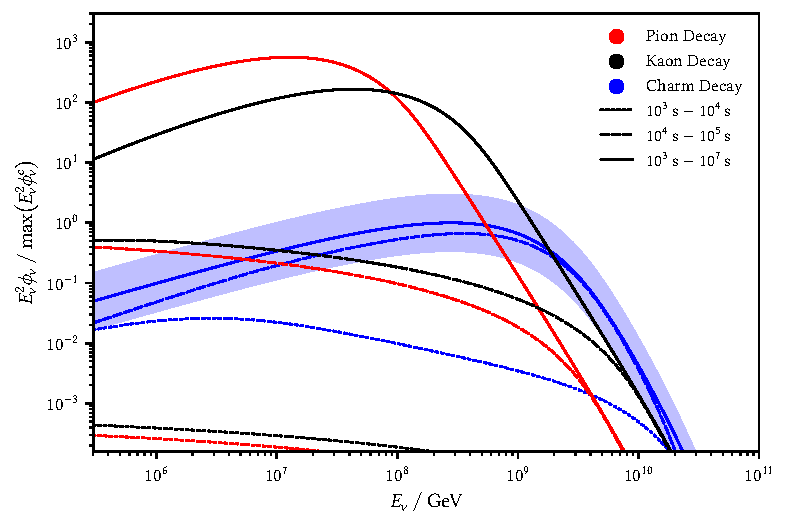
\includegraphics{../plots/build/magnetar_integrated_neutrino_spectrum_without.pdf}
	\caption[Magnetar $\nu \kern+0.5pt$ fluence compared to $c$ decay without optical depth.]
			{Expected neutrino fluence weighted by the charm contribution from a young magnetar for different time
			 intervals after formation, excluding the optical~depth defined by \eqref{eqn:optical} as a modification.
			 In agreement with prior expectations derived from Sections \ref{sub:spindown} and \ref{sub:charm} for energy
			 scaling and mean lifetimes, respectively, first pion, then kaon, and eventually charm dominate, sorted
			 by increasing energy. The same shaded uncertainty band as in Figure \ref{fig:magnetar-flux-with}
			 for charm decays as well as the scaling by $E_\nu^2$ from Figure \ref{fig:magnetar-fluence-with} are adopted.
			 With charmed hadrons being significant beyond $E_\nu = \kern-0.5pt \qty{e9}{\giga\electronvolt}$ and their lower
			 uncertainty bound never exceeding the kaon curve, it is unclear if substantial charm signals are likely.}
	\label{fig:magnetar-fluence-without}
\end{figure}
